\section{Back-Face Culling} The more polygons we have to draw, the more slower
our execution of the program gets. In order to cut down on the expensive
operations went want a method that sorts out the surfaces of our cube, that are
not visible. For that we use Back-Face culling. BFC is a method to determine
whether a given surface is visible. More specifically it's a way to determine
if a polygon of an object is occluded.

To achieve this two vectors are needed. The normal on the surface of the object,
and the vector from the camera center to the object surface. The angle between
these two vectors determine weather the surface is viewable from the camera's
view point. As the angle increases, the surface reaches a point where its only
visible as a line, and after that we only see the back side of the surface, and
it should no longer be drawn.

The orthonormal of the object surface can be found by the cross product of the
surface's standard basis. For cube's faces, this is easily defined as two
vectors between the corners (avoiding diagonals), if we relax the claim of
orthonormality to that of orthogonality.
\begin{figure}[hbtp]
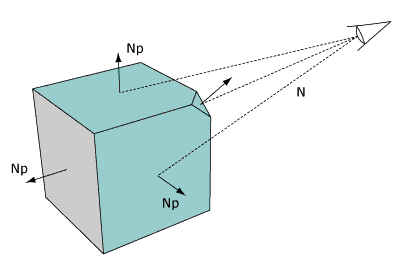
\includegraphics{pics/culling.png}
\label{fig:culing}
\caption{Normals (denoted Np) of a cube's faces, and the vectors from the camera
center to the centers of those faces)}
\end{figure}
